\documentclass[10pt]{article}

\usepackage{graphicx}
\usepackage{float}
\usepackage{amsmath}
\usepackage{amssymb}
\usepackage{multicol}
\graphicspath{{Images/}}

\addtolength{\oddsidemargin}{-.7in}
\addtolength{\evensidemargin}{-.7in}
\addtolength{\textwidth}{1.75in}
\addtolength{\topmargin}{-.7in}
\addtolength{\textheight}{1.75in}

\setlength{\columnsep}{1cm}

\begin{document}
\author{ David Strachan and Edward Gandar }
\title{\textbf{Dipolar BEC simulations}}

\maketitle

\tableofcontents

\pagebreak

\begin{multicols}{2}

\section{The Gross-Pitaevskii equation (GPE) for dipolar condensates in three dimensions}

At ultra-low temperatures the properties of a dipolar condensate with $N$ atoms, each of mass $m$, can be described by the GPE below.

\begin{multline}
i\hbar \frac{\partial \psi(\textbf{r},t)}{\partial t}=\bigg[-\frac{\hbar^2}{2m}\nabla^2 + V_{ext}(\textbf{r}) + \frac{4\pi \hbar^2 a_{s} N}{m}|\psi(\textbf{r}',t)|^2 \\+ N \int_V U_{dd}(\textbf{r}-\textbf{r}')|\psi(\textbf{r},t)|^2d^3\textbf{r}' \bigg]\psi(\textbf{r},t)
\end{multline}

where $\int_V d^3\textbf{r} |\psi(\textbf{r},t)|^2 = 1$ and $a_{s}$ is the atomic s-wave scattering length. The trapping potential is assumed to be either in the form $$V_{ext}=\frac{1}{2}m(w^2 x^2+w^2 y^2+w_{z}^2z^2)$$ and is assumed to have cylindrical symmetry about the z axis, or a circle box potential,
$$V_{ext}=0$$ for $r<R$ in the radial direction and infinite elsewhere and $$V_{ext}=\frac{1}{2}mw_{z}^2z^2$$ harmonic in the z axis. Where $w$ is the angular frequency.

The dipolar interation, for magnetic dipoles, is described by the equation:
\begin{equation}
U_{dd}(\textbf{r}-\textbf{r}') = \frac{\mu_{0} \bar{\mu}^2}{4\pi} \frac{1-3 cos^2(\theta)}{|\textbf{r}-\textbf{r}'|^3}
\end{equation}
where $\theta$ is the angle between $\textbf{r}-\textbf{r}'$ and the direction of the polarization, chosen to be z, $\mu_{0}$ is the permeability of free space, and $\bar{\mu}$ is the dipole moment of the atom.

Going into dimensionless units, $t \Rightarrow \frac{t}{\omega}, \textbf{r} \Rightarrow x_{s}\textbf{r}$ with $x_{s}=\sqrt{\frac{\hbar}{m\omega}}$, $\psi \Rightarrow \ \psi x_{s}^\frac{-3}{2}$ we end up with the equation
\begin{multline}
i\frac{\partial \psi(\textbf{r},t)}{\partial t}=\bigg[-\frac{1}{2}\nabla^2 + \frac{1}{2}(x^2+y^2+\gamma z^2) + g_{s}|\psi(\textbf{r},t)|^2 \\+ D \int_V U_{dd}(\textbf{r}-\textbf{r}')|\psi(\textbf{r}',t)|^2d^3\textbf{r}' \bigg]\psi(\textbf{r},t)
\end{multline}

where $g_{s}=\frac{4 \pi a_{s} N}{x_{s}}$, $\gamma=\frac{w_{z}}{w}$ is the trap ratio and $D=\frac{m N \mu_{0} \bar{\mu}^2}{4 \pi \hbar^2 x_{s}}$.



\section{Basic strucure of code with no interactions in cartesian coordinates}
This is a very basic and quickly put together summary of our methods, it's not thorough and can easily be expanded and more detailed. In terms of the comparison between the codes that you mentioned in the email,we haven't finished various parts of the code and are having various issues, but I think we should be able to do this within the next week. This only covers the harmonic case and obviously the hard wall potential is likely more important, but the structures are very similar and we've mainly been working with the harmonic case more recently. Lots of the issues/structure of the code apply to both cases.

Firstly, all the parameters (number of points, frequency etc) are defined at the start and can easily be adjusted. For 1D, a linear array is defined from over the range in position space wanted, and a linear array in k space is defined using the fftfreq function. For higher dimensions, these are simply repeated over the other dimensions with y and z arrays defined in the same way but along the different axes. We convert into dimensionless units using the length scale $x_{s}$ which leads to 
\begin{equation}
V(r) = \frac{1}{2}x^{2}+\frac{(\gamma_yy)^{2}}{2}+\frac{(\gamma_zz)^{2}}{2}
\end{equation}
and the kinetic term is defined in k space as 
\begin{equation}
T(k) = \frac{1}{2}k^{2}
\end{equation} 
We use an initial guess of a gaussian but this can be any function that is non zero at the origin and is symmetric. The split step fourier method is then used with imaginary time propagation, and after each iteration $\psi$ is normalised. This repeats until convergence, and the solutions are plotted against the true ground state.
\section{Contact and dipolar interactions}
The contact interaction term is very simple to code, the potential becomes 
\begin{equation}
V(r) = \frac{1}{2}r^{2}+g_{s}|\psi|^{2}
\end{equation}
Before every step $\psi$ is normalised to ensure terms that are functions of $\psi$ have the same weighting.
 
The dipolar term involves integrating $U_{dd}$ with $|\psi|^{2}$ over all space, which can be treated as a convolution. This is easily evaluated in k space, and we code it as a function. We introduce a spherical cut off in position space to prevent alias copies, which leads to the following expression in k space 
\begin{equation}
\tilde{U_{dd}}(k) = \frac{Cdd}{3}[1+3\frac{\cos(R_{c}k)}{(R_{c}k)^{2}}-3\frac{\sin(R_{c}k)}{(R_{c}k)^{3}}](3\cos{\theta_{k}}^{2}-1)
\end{equation} 
This works for near-spherical traps, but if the trap is pancake like, a cylindrical cut off is needed. This leads to
\begin{multline}
\tilde{U_{dd}}(k) = \frac{C_{dd}}{3}(3\cos{\theta_k}^{2}-1) \\+ C_{dd}e^{-Z_{c}k_{\rho}}[\sin{\theta_{k}}^{2}\cos{Z_{c}k_{z}} -\sin{\theta_{k}}\cos{\theta_{k}}\sin{Z_{c}k_{z}}] \\- C_{dd}\int_{\rho_{c}}^{\infty}\rho d\rho\int_{0}^{Z_{c}}dz\cos{k_{z}z}\frac{\rho^{2}-2z^{2}}{(\rho^{2}+z^{2})^{\frac{5}{2}}}J_{0}(k_{\rho}\rho),
\end{multline} 
Where $J_{0}(x)$ is the zeroth order bessel function of the first kind.

The potential becomes
\begin{equation}
V(r) = \frac{1}{2}r^{2}+g_{s}|\psi|^{2}+\psi_{cont}(\psi)
\end{equation}
where 

\begin{equation}
\psi_{cont}(\psi) = F^{-1}(\tilde{U_{dd}}(k)|\psi(k)|^{2})
\end{equation}
\section{Hankel Transform}
If the dipole polarisation is along the z axis, the ground state will be cylindrically symmetric in a harmonic trap (or circular box potential). This can reduce a 3D system to an effective 2D system, where only the r and z coordinates are needed. If we are in cylindrical coordinates, the space where the r component of the Laplacian operator is diagonalised is bessel space. To transform from position space to bessel space, we use a Hankel transform. In ref \cite{Kai_Ming_2009} they outline a very efficient method to compute a discrete Hankel transform for a finite range of r. First, we rewrite the function in both position space $f(r)$ and bessel space $g(\rho)$ as a Dini series. If $0<r<b$ and $0<\rho<\beta$ then we can write f(r) and $g(\rho)$ as
\begin{equation}
f(r) = \frac{2}{b^{2}}\sum_{n=0}^{\infty}f_{n}J_{0}^{-2}(\alpha_{n})J_{0}(\frac{\alpha_{n}r}{b})
\end{equation}
\begin{equation}
g(\rho) = \frac{2}{\beta^{2}}\sum_{n=0}^{\infty}g_{n}J_{0}^{-2}(\alpha_{n})J_{0}(\frac{\alpha_{n}\rho}{\beta})
\end{equation}
where 
\begin{equation}
f_{n} = \int_{0}^{b}rf(r)J_{0}(\frac{\alpha_{n}r}{b})dr=\frac{1}{2\pi}g(\frac{\alpha_{n}}{2\pi b})
\end{equation}
and
\begin{equation}
g_{n} = \int_{0}^{\beta}\rho g(\rho)J_{0}(\frac{\alpha_{n}\rho}{\beta})d\rho=\frac{1}{2\pi}f(\frac{\alpha_{n}}{2\pi\beta})
\end{equation}
where $\alpha_{n}$ are the real nonnegative roots of the derivative of the zero-order Bessel function, $\alpha_{0}=0$. We can truncate these infinite sums to finite ones by using the fact that if $\alpha_{N} >S$ where $S=2\pi b\beta$, both $f_{N}$ and $g_{N}$ are zero.

Defining a change of variables, 
\begin{equation}
G(m) = g(\frac{\alpha_{m}}{2\pi b})|J_{0}^{-1}(\alpha_{m})|\beta
\end{equation}
\begin{equation}
F(n) = f(\frac{\alpha_{n}}{2\pi \beta})|J_{0}^{-1}(\alpha_{n})|b
\end{equation}
leads to the following formula for the discrete Hankel transform and its inverse,
\begin{equation}
G(m) = \sum_{n=0}^{N}c_{mn}F(n)
\end{equation}
\begin{equation}
F(n) =  \sum_{n=0}^{N}c_{nm}G(m)
\end{equation}
where $c_{nm}$ are the elements of a transform matrix, 
\begin{equation}
c_{nm} = \frac{2}{S}|J_{0}^{-1}(\alpha_{n})||J_{0}^{-1}(\alpha_{m})|J_{0}(\frac{\alpha_{n}\alpha_{m}}{S})
\end{equation}
For this to hold, the matrix C has to satisfy $CC =I$, and C is a function of S only so S must be chosen correctly. In \cite{Kai_Ming_2009} they state that the optimum choice is 
\begin{equation}
S = 2|J_{0}^{-1}(\alpha_{k})|\sqrt(1+\sum_{n=1}^{N}J_{0}^{-2}(\alpha_{n})J_{0}^{2}(\frac{\alpha_{k}\alpha_{n}}{J_{N+1}}))
\end{equation}
where 
\begin{equation}
k = Int(\frac{N}{4})
\end{equation}
Despite redefining S in a different way, as long as $S<\alpha_{N+1}$, this approach is still valid.


 To code this, we  define C and S along with N at the start so we only need to run this when we want to change N. Then we simply replace the fft2 function by this transform and the code runs the same.
\section{Using Hankel transform in 3D}

In 3D, we reshape the r array to be 2D, repeating along the 2nd axis and create a 2D z array which repeats over the other axis. The main difference is within the loop. We apply half the potential on position space, then apply the fourier transform alone the z axis and the hankel transform along the r axis. We then apply the kinetic term. Finally, we transform back to position space and apply the second half of the potential. This is then iterated until convergence. 

 Further efficiency can be achieved by realising all solutions will be symmetric in z, so only $z\geqslant0$ so instead of using a fourier transform we can use a fast cosine transform, which leads to faster computation.

\section{Quasi 2D approach}
When the axial trap is very strong, a good approximation to make is that the BEC in the axial direction is confined to the axial ground state REFERENCE CPC PAPER
 \begin{equation}
\phi(z) = \frac{1}{(\pi\epsilon)^{\frac{1}{4}}}e^{\frac{-z^{2}}{2\epsilon}}, \epsilon = \frac{1}{\gamma}
\end{equation}
We then take the ansatz 
 \begin{equation}
\psi(r,z) = \psi_{2D}(\textbf{x}_{\perp})\phi(z),
\end{equation}
and inserting this into Eq(3), multiplying by $\phi(z)$ and integrating over z we get the the following quasi 2D GPE




\begin{multline}
i\frac{\partial \psi_{2D}(\textbf{x}_{\perp},t)}{\partial t}=\bigg[-\frac{1}{2}\nabla_{\textbf{x}_{\perp}}^2 + \frac{1}{2}(x^2+y^2) \\+\frac{g_{s}}{\sqrt{2\pi\epsilon}}|\psi_{2D}(\textbf{x}_{\perp},t)|^2
+\frac{4\pi D}{3}\\\cdot\int d\textbf{k}_{x_{\perp}}e^{-2\pi i\textbf{k}_{x_{\perp}}\cdotp \textbf{x}_{\perp}}\tilde{n}(\textbf{k}_{x_{\perp}},t)h_{2D}(\xi)\bigg]\psi_{2D}(\textbf{x}_{\perp},t),
\end{multline}
where 
\begin{multline}
\tilde{n}(\textbf{k}_{x_{\perp}},t) = \int d\textbf{x}_{\perp}e^{2\pi i\textbf{k}_{x_{\perp}}\cdotp \textbf{x}_{\perp}}|\psi_{2D}(\textbf{x}_{\perp},t)|^2,
\end{multline}

\begin{multline}
h_{2D}(\xi)=\frac{1}{\sqrt{2\pi\epsilon}}[2-3\sqrt{\pi}exp(\xi^2)erfc(\xi)],              
\end{multline}
\begin{equation}
\xi = k_{x_{\perp}}\sqrt{\frac{\epsilon}{2}}.             
\end{equation}
This is very similar to the orginal GPE in structure, the only difference being the reduced dimension and the modified terms. We have assumed cylindrical symmetry so a Hankel transform can be used, reducing a 3D problem to a 1D one. 

This method achieves very accurate results of within $0.001\%$ of the true ground state with no interactions.
\begin{figure}[H]
\centering
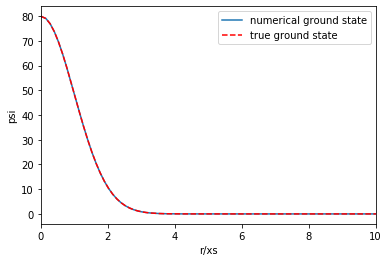
\includegraphics[width=0.6\linewidth]{gndstateQuasi2DHankel}
\caption{Comparison of the harmonic ground state and the numerical solution using the Quasi 2D Method}
\end{figure}


\section{Accuracy with no interactions}
In 3D, the ground state wavefunction with no interactions is shown below:

\begin{figure}[H]
\centering
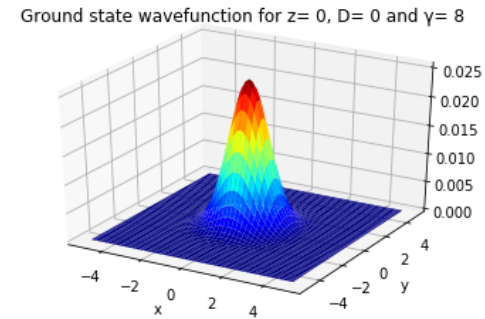
\includegraphics[width=0.6\linewidth]{gndstate1}
\caption{Ground state with $\gamma=8$}
\end{figure}

An error of ~0.3\% is achieved.

ADD RED BLOOD CELL GRAPH

In 3D using a hankel transform and a cosine fast transform, we achieve the same ground state within $0.008\%$ of the true ground state with no interactions.

\begin{figure}[H]
\centering
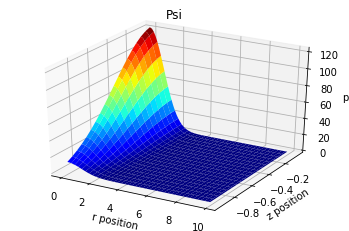
\includegraphics[width=0.6\linewidth]{gndstate3DHankel}
\caption{Ground state with $\gamma=5$ using the Hankel transform and cosine transform}
\end{figure}


	
Using the Hankel transform in 2D (1D computationally), we achieve very accurate results compared to the harmonic oscillator ground state.
INSERT GRAPHS HERE
Using the 2d fourier transform, we also achieve very accurate results.
INSERT GRAPHS HERE


\section{Thomas Fermi}
The Thomas Fermi radius for a given axis is given by 
\begin{equation}
R_{i} = \sqrt{\frac{2\mu}{m\omega_{i}^2}},
\end{equation}
\begin{equation}
\mu = \frac{\hbar\bar{\omega}}{2}\bigg(\frac{Na}{x_{s}}\bigg)^{\frac{2}{5}},
\end{equation}
where $\omega_{i}$ is the harmonic frequency along that axis and $\mu$ is the chemical energy. 
DO CONTACT THOMAS FERMI AND THOMAS FERMI FROM QUASI 2D AND 1D PAPER

\section{Contact interactions}
A good check for validity is whether our solutions agree with the analytical solution in the Thomas-Fermi regime. Firstly, we compare our Quasi 2D solution with the analytical solution and we see we achieve very high accuracy.

 
\begin{figure}[H]
\centering
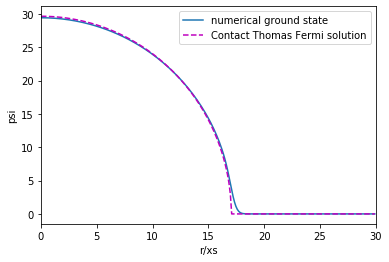
\includegraphics[width=0.6\linewidth]{ContactThomasFermiQuasi 2DHankelgamma=50No=4e5}
\caption{Thomas fermi regime with gamma = 50, N=4e5, using the Quasi 2D approach}
\end{figure}

We now compare our full 3D solution using the Hankel transform and the fast cosine transform, 

\begin{figure}[H]
\centering
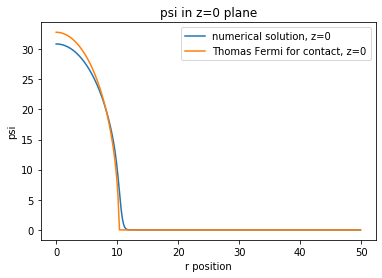
\includegraphics[width=0.6\linewidth]{Contact Thomas Fermi 3D Hankel gamma=5 No=2e5}
\caption{Thomas fermi regime with gamma = 5, N=2e5, using the 3D Hankel approach}
\end{figure}

The discrepancies between the analytical solutions and our solutions may be due to the fact that the Thomas-Fermi solution is only valid up to the edges of the cloud, where the Thomas-Fermi approximation becomes discontinous. With 3D the normalisation might be slightly wrong which is why the radius seems correct but the magnitude is slightly off.
\section{Purely dipolar interactions}
The extension of the Thomas-Fermi analysis remains valid in a purely dipolar condensate with modified terms, and when the Quasi 2D approximation becomes valid this becomes especially simple. This is because the dipolar interaction can be rewritten as a short-range term and a long-range one, and when the condensate is strongly defined in the axial direction this long-range term can be neglected aswell as the kinetic term.

I  
 
\begin{figure}[H]
\centering
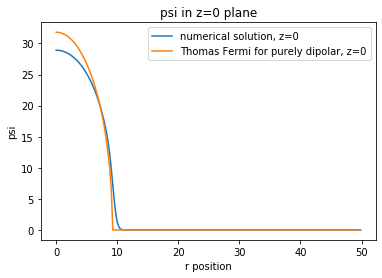
\includegraphics[width=0.6\linewidth]{Dipolar Thomas Fermi 3D Hankel gamma = 80 No=2e4}
\caption{Dipolar Thomas-fermi regime with gamma = 80, N=2e4, using the 3D Hankel approach}
\end{figure}

\begin{figure}[H]
\centering
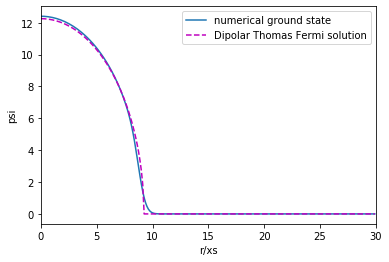
\includegraphics[width=0.6\linewidth]{Dipolar Thomas Fermi Quasi 2D Hankel gamma = 80 No = 2e4}
\caption{Dipolar-Thomas fermi regime with gamma = 5, N=2e5, using the Quasi 2D approach}
\end{figure}

\section{Discussion of stability of a purely dipolar gas}

\subsection{In a harmonic trap}

In general, the higher the trap ratio ($\lambda$), the more dipoles are required to make the condensate unstable. (This is due to fewer dipoles above or below any given dipole, since the dipole force is attractive in the cone above a dipole). Eventually, the BEC always becomes unstable for a large enough number of particles (for a given $C_{dd}$).

I need to label the colours and axis on this graph, white and black represent stable and unstable regimes respectively. Red represents the regime where bioconcave ground states are achieved. I think the red streaks are due to the grid resolution being too low.

\begin{figure}[H]
\centering
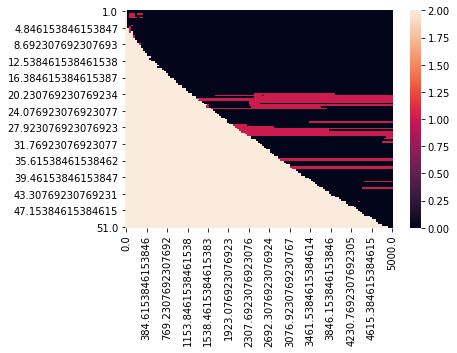
\includegraphics[width=0.6\linewidth]{stability plot dt =0.005}
\caption{Stability plot of gamma against the dimensionless parameter D,I need to label the colours and axis on this graph, white and black represent stable and unstable regimes respectively. Red represents the regime where bioconcave ground states are achieved. I think the red streaks are due to the grid resolution being too low.}
\end{figure}

\subsection{In a pancake trap}

 In a similar fashion to the harmonic trap, we define the dimensionless dipole interation parameter, $D=\frac{NmCdd}{\hbar^{2}x_{s}}$ where $ x_{s} =L$ is the size of the trap.
 
 
 \end{multicols}


\bibliographystyle{unsrt}
\bibliography{references}
 
%\begin{equation}
%i \frac{\partial \psi(r,t)}{\partial t}= \left(-\frac{1}{2} \nabla^2+\frac{1}{2}r^{2}+\beta_{2D}|\psi|^{2}-\frac{3\lamda}{2}(\partial_{nn}-n_{3}^{2}\nabla^{2})((-%\nabla^{2})^{-\frac{1}{2}}|\psi|^{2})) \psi(r,t),
%\end{equation}


\end{document}